\subsection{Multipole-to-Multipole (M2M)}
At this point in our octree, all leaf nodes have multipole expansions.

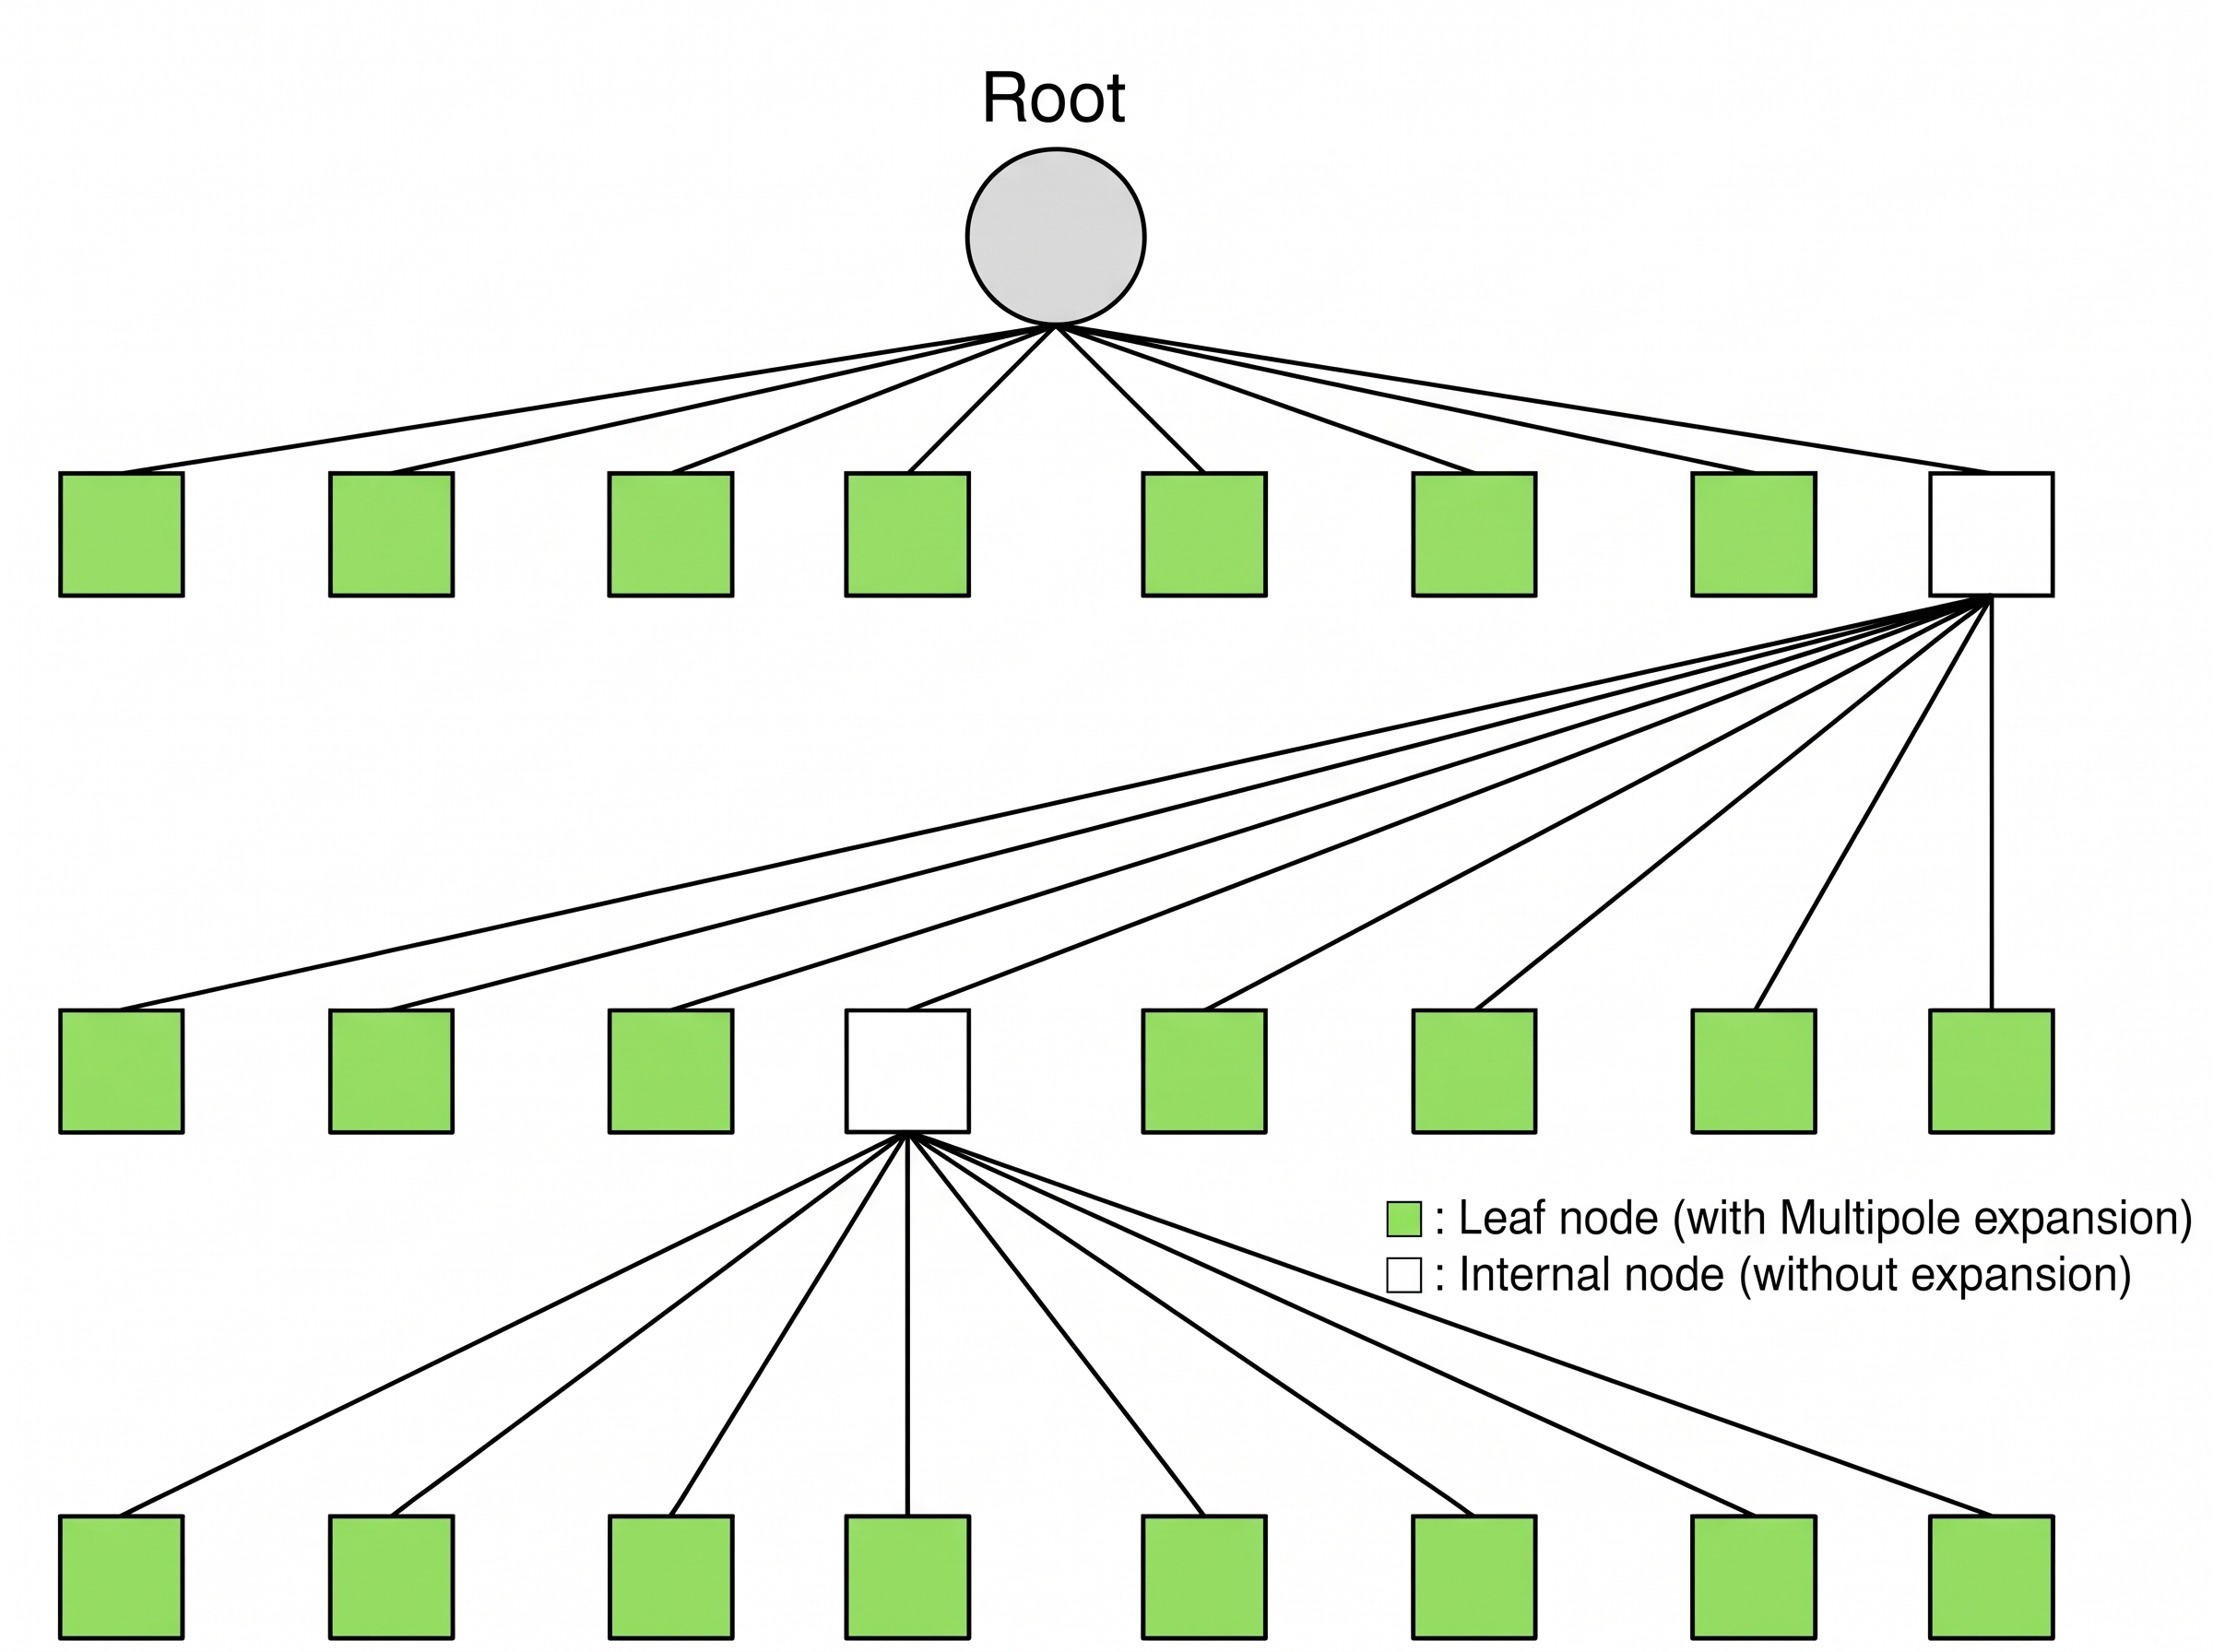
\includegraphics[width=\linewidth]{sections/images/Octree_P2M.png}

\subsubsection{Implementation}
We now move from the bottom level to the top, processing the internal nodes in parallel.

\begin{lstlisting}[language=C]
const int max_level = level_bounds.size() - 2;

for (int level = max_level - 1; level >= 0; level--) {
        const int level_start = level_bounds[level];
        const int level_end = level_bounds[level + 1];
        const int num_nodes_in_level = level_end - level_start;

        if (num_nodes_in_level == 0) continue;

        m2mKernel<<<num_nodes_in_level, kBlocksize>>>(...);
\end{lstlisting}

Here, \texttt{level\_bounds} stores the starting index of each level (for example, level 2 may start at node 35). Its last element is the total number of nodes in the octree. Therefore, we subtract 2 from its length to get the index of the deepest level: one position is used for the final total-node count, and indexing starts at 0.

We then iterate from the deepest level up to level 0. For each level, we launch one block per node, so each node gets one block to perform its M2M translation.

\subsubsection{Inside an M2M kernel}

We allocate shared memory for the regular harmonics of all eight children, \(R_l^m\).

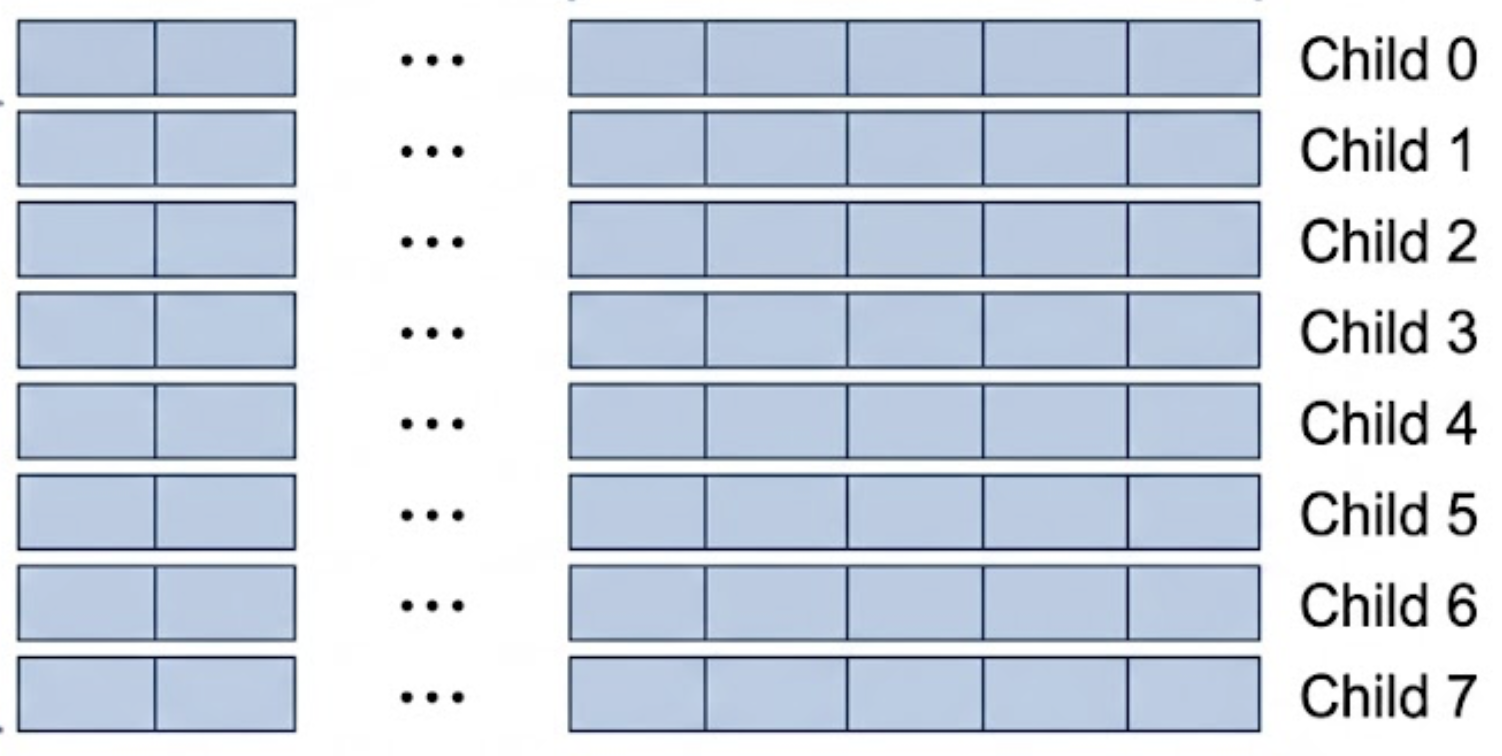
\includegraphics[width=\linewidth]{sections/images/shared_memory_for_child_harmonics.png}

Threads 0 through 7 each compute the regular harmonics for one child and store them in rows 0 through 7.

\subsubsection{Translation formula}

Let the parent center be \(\mathbf{c}_p\) and the center of child \(c\) be \(\mathbf{c}_c\), where \(c=1,\ldots,8\). The displacement from the parent center to the child center is

\[
\mathbf{d}_{cp}
= \mathbf{c}_c
-
\mathbf{c}_p
\]

For each child, we compute the regular harmonics \(R_l^m\):

\[
\mathbf R=
\begin{bmatrix}
R_{00}^{(1)} & R_{10}^{(1)} & \cdots & R_{10,10}^{(1)}\\
R_{00}^{(2)} & R_{10}^{(2)} & \cdots & R_{10,10}^{(2)}\\
\vdots & \vdots & \ddots & \vdots\\
R_{00}^{(8)} & R_{10}^{(8)} & \cdots & R_{10,10}^{(8)}
\end{bmatrix}
\]

For a parent coefficient of degree \(l\) and order \(m\), the translation theorem gives

\[
M_{lm}^{(P)}
=
\sum_{c=1}^{8}
\sum_{j=0}^{l}
\sum_{\substack{k=-j\\|m-k|\le l-j}}^{j}
M_{jk}^{(c)}
\overline{R_{l-j}^{m-k}(\mathbf d_{cp})}
\]

For negative-order multipoles, we use the symmetry relation below for \(m>0\):

\[
M_{l}^{-m}
=
(-1)^{m}
\overline{M_{l}^{m}}
\]